\chapter{Conclusions}


\section{Summary of Contributions}


 
The scientific objectives of this thesis, as they were described in Section \ref{sec:objectives}, are:

\begin{enumerate}
	\item The development of methods for the characterization of acoustic parameters.
	\item The research on parametric-based methodologies for sound event localization and detection.
	\item The contribution in the generation and storage of annotated ambisonic datasets.
\end{enumerate}

In the following list we provide the main contributions of the present thesis, both in the academic and software scopes. Contrubitions are organized by the Chapter where they appear; the index of the respective contribution is also indicated:
  
  \begin{itemize}

  	 \item Blind reverberation time estimation (Chapter~\ref{chap:rt60}):
  	\begin{description}
  		\item [1. Parameter estimation] Novel technique for blind RT60 estimation of ambisonic recordings from autoregressive models.
	\end{description}

  
  	\item Coherence estimation (Chapter~\ref{chap:coherence}):
  	\begin{description}
  		\item [1. Parameter estimation] Contribution to the characterization of coherence with tetrahedral microphones (the most common spherical arrangement).
	\end{description}


  	\item Sound Event Localization and Detection (Chapter~\ref{chap:seld2019}):
  	\begin{description}
  		\item [2. Scene Description]: Novel state-of-the-Art methodology for Sound Event Localization and Detection	.
  	\end{description}
  	
  	\item Data generation and storage (Chapter~\ref{chap:data}):
  		\begin{description}
  			\item [3. Data Generation]: Library for acoustic simulation and spherical microphone array processing.
  			\item [3. Data Generation]: Proposal and implementation of a file convention for the storage of recorded ambisonic RIRs.
  			\item [3. Data Generation]: Novel tool for high-level description and generation of of ambisonic datasets.

 		\end{description}

  \end{itemize}
  
   
Figure~\ref{fig:scheme1_numbers2}, which is a copy of Figure~\ref{fig:scheme1_numbers}, 
 has been included here again in order to help the contextualization of the contributions. 

  \begin{figure}[h!]
  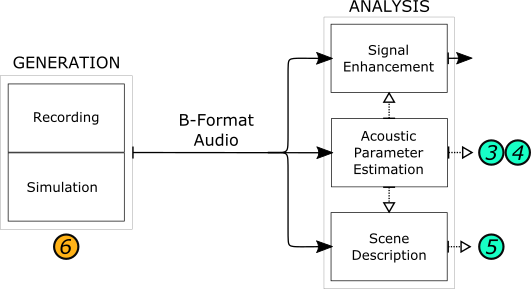
\includegraphics[width=\textwidth]{Figures/Introduction/SCHEME1_NUMBERS.png}
  \caption{General scheme of the B-Format audio generation and analysis framework, including the thesis contributions in form of Chapter numbers.}
  \label{fig:scheme1_numbers2}
\end{figure}




\section{Conclusion and Future Work}

This thesis has tackled several research problems associated with the analysis of ambisonic recordings, making use primarily of the parametric sound field modelling.
Chapter~\ref{chap:rt60} presents a novel methodology for the blind estimation of reverberation time from ambisonic audio. The method is based on two main steps: first, dereverberation using a multichannel auto-recursive model (MAR), and second, estimation of the  filter from reverberant and dereverberated signals. The actual reverberation time value is estimated from the energy decay of the estimated filter. 

The proposed system is the first attempt in the literature to address the blind reverberation time estimation problem specifically for ambisonic signals. Compared with a state-of-the-art monophonic estimator, our method is able to improve in all the standard evaluation metrics under consideration.

Still, there is much room for improvement. Among others, the method could be easily extended to higher order ambisonic signals, which might still improve the reported results due to the availability of much more audio channels. Moreover, the usage of online MAR methods would enable the possibility of analyzing sound scenes with moving sources; the statistical time-invariance property of late reverberation supports this hypothesis. Finally, it is important to mention that the proposed method is resource-intensive. An analysis of the trade-off between computation time and evaluation performance, mostly dependent on the estimation filter length, remains to be done.  

Given the current interest in the field of augmented reality, new related research topics emerge. One of them, which has been recently baptized as \textit{acoustic matching} \cite{su2020acoustic}, deals with the analysis of acoustic properties of real enclosures, with the aim of later introduction of virtual elements whose reverberation would match real conditions. 
The application of our method to the acoustic matching problem is straightforward: given an ambisonic recording with a target reverberation, estimate its reverberation time and synthesize a reverberant tail with the target energy decay; early reflections might be generated by various methods, including physical models or perceptually motivated approaches. 
We can foresee a growing interest on the topic in the near future; our contribution might help to establish the foundation of a new family of methods. \\


In Chapter~\ref{chap:coherence}, we have characterised the response of tetrahedral microphones to isotropic noise field, which is one of the most used models for diffuse sound. Furthermore, the capabilities of a spherical loudspeaker array with respect to the reconstruction of diffuse sound fields using ambisonics are also tested. 
Future work in this direction might include the characterisation of different spherical microphone array geometries, and different types of diffuse field models. Additionally, the loudspeaker array diffuse field reconstruction experiment could be easily extended. \\


Chapter~\ref{chap:seld2019} describes an algorithm for sound event localization and detection (SELD), developed in the context of the DCASE 2020 challenge. The method estimates the localization and temporal activity of the sound events based on a particle filter that tracks event trajectories obtained from the parametric analysis of the ambisonic sound field. Each event is assigned to a sound class by a machine learning classifier that uses low- and mid- level audio features. Results on the cross-validation development set show a significant performance increase in most evaluation metrics, compared with a state-of-the-art deep learning baseline. This result shows that our approach, which is substantially different to the baseline and the majority of state-of-the-art methods, represents an alternative in specific situations with low-complexity or small database constraints. 

The wide scope of the SELD task allows for a wide range of research continuation possibilities. For instance, one of the major problems of the proposed algorithm is the inaccurate parametric estimation when two events are simultaneously active. Although it is a known problem in the literature, a successful solution in the given context remains still to be found.

Another source of potential improvements is the refinement of the particle filter applied to this specific task. A deeper understanding of control theory, as well as collaborations with experts on the field, might bring a noticeable improvement on the overall system performance.

The performance of the event classifier might be also further analyzed. Although in this case we opted for a classical feature-based machine learning approach, different methods and architectures could be compared, including more modern deep-learning approaches.\\

Finally, the thesis contributions to more practical aspects are presented in Chapter~\ref{chap:data}. Those contributions comprise two software libraries written in Python: one of them focused on spherical microphone array and acoustic simulation, and another one implementing the SOFA standard, which has also been revised and modified for allowing the representation of ambisonic data. Finally, a software for the procedural creation of annotated reverberant ambisonic datasets has ben also presented. 

Apart from the straightforward task of software maintenance, the engagement of the research community with the usage and eventual contribution of the libraries would represent a desired situation in the near future. Moreover, the proposed file format convention is being currently discussed for its adoption into the SOFA standard, which can be considered an achievement of the original proposal. 
 
